\documentclass[10pt]{article}
\usepackage{icmlko}

\icmlmeta{IP 파운데이션 월드모델}{153}{평균 내지 말고 읽었더니}{노트 152가 ``공유 다섯은 태거가 제일 못 읽는 다섯''이라 했다. 임베딩을 평균하는 대신 문서를 읽혔더니 그 다섯이 $\rho$ 0.236에서 0.774로 올랐다}

\begin{document}

\twocolumn[
\icmlheader

\begin{abstract}
노트 151이 팝업 표본의 벽을 ``사람이 축을 매긴 건수''로 좁혔고, 노트 152가
자동 태거를 열어 \textbf{우리가 쓰는 공유 다섯이 태거가 제일 못 읽는 다섯}
임을 보였다(태거 $\rho$ 평균 0.236). 지금 태거는 문장 임베딩을 24차원으로
줄여 능형에 넣는다. 그런데 ``매장이 얼마나 눈에 띄나''는 임베딩 평균으로
잡히는 종류가 아니다 --- \emph{읽어야} 나온다. 그래서 읽어 봤다.
사람이 매긴 팝업 26건을 뽑아 \textbf{기획 문서만 보고}(사람 라벨도 결과값도
안 보고) 같은 0$\sim$4 루브릭으로 직접 매겼다. \textbf{공유 다섯 평균
$\rho$ 가 0.236에서 0.774로 오른다.} 다섯 축 전부 오르고, 제일 크게 오른
것이 미디어 푸시($0.249\to0.911$)와 타깃 폭($0.151\to0.837$)이다. 평균
절대오차는 0.927에서 0.515로 \textbf{45\% 준다}(0$\sim$4 척도에서). 노트
152가 세운 운영 사실 --- ``지금 태거로는 팝업 표본을 못 늘린다'' --- 의
``지금 태거로는''이 핵심이었던 셈이다. \textbf{그런데 바로 채택하지 않는다.}
적용할 대상이 다르다. 축이 안 매겨진 108건 중 107건이 \emph{시장 레코드}
(기사에서 뽑은 외부 사례)이고, 그 문서의 중앙 길이가 \textbf{158자}다 ---
사람이 매긴 81건의 676자에 견주면 4분의 1이다. 그리고 내 오차는 문서가
얇을수록 커진다(길이와 오차의 순위상관 $-$0.335, 긴 절반 MAE 0.369 대 짧은
절반 0.662). \textbf{그러므로 $\rho{=}0.774$ 는 676자짜리 문서에서 잰
값이고 158자에서도 그렇다는 보장이 없다.} 다음 할 일이 정확히 과제 78이고,
이제 그 과제가 왜 필요한지도 분명하다.
\end{abstract}
]

\begin{figure*}[t]
\centering
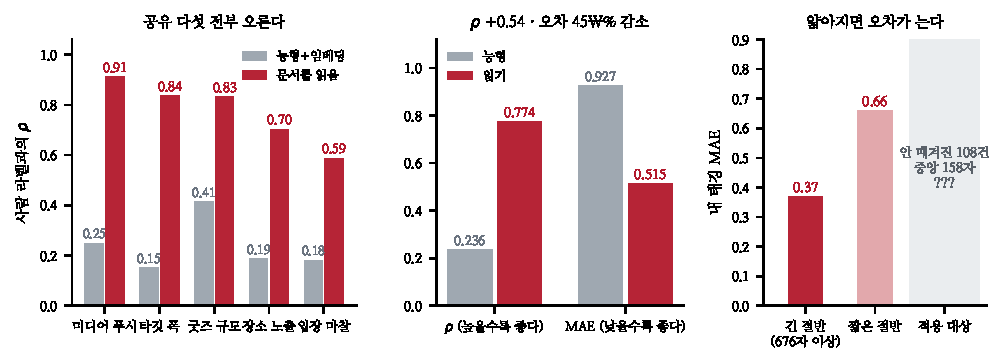
\includegraphics[width=\textwidth]{figs/llm.pdf}
\caption{왼쪽 --- 공유 다섯 전부 오른다. 가운데 --- $\rho$ $+$0.54, 오차
45\% 감소. 오른쪽 --- 문서가 얇아지면 오차가 는다.}
\end{figure*}

\section{설계 --- 눈가림}

사람이 매긴 팝업 67건에서 26건을 씨앗 고정으로 뽑고, 각 건의 기획 문서만
꺼냈다(\texttt{autotag.read\_plan} 이 결과값을 딕셔너리에서 아예 지운다).
\textbf{사람 라벨도 결과값도 보지 않은 상태에서} 공유 다섯을 0$\sim$4로
매기고, 그 다음에 붙여서 채점했다.

\begin{table}[t]
\centering\tsize
\caption{사람 라벨과의 일치. 26건.}
\begin{tabular}{lrrrr}
\toprule
& \multicolumn{2}{c}{$\rho$} & \multicolumn{2}{c}{MAE} \\
& 능형 & \textbf{읽기} & 능형 & \textbf{읽기} \\
\midrule
미디어 푸시 & .249 & \textbf{.911} & .830 & \textbf{.423} \\
타깃 폭 & .151 & \textbf{.837} & .955 & \textbf{.538} \\
굿즈 규모 & .414 & \textbf{.832} & .964 & \textbf{.346} \\
장소 노출 & .187 & \textbf{.703} & .733 & \textbf{.462} \\
입장 마찰 & .181 & \textbf{.587} & 1.153 & \textbf{.808} \\
\midrule
\textbf{평균} & \textbf{.236} & \textbf{.774} & \textbf{.927} & \textbf{.515} \\
\bottomrule
\end{tabular}
\end{table}

\claimx{\textbf{다섯 축 전부 오르고 평균이 $+$0.538이다.} 제일 크게 오른
것이 미디어 푸시($+$0.662)와 타깃 폭($+$0.686) --- 노트 152에서 태거가
제일 못 읽던 둘이다.}{$n{=}26$ 이라 $\rho$ 의 표준오차가 0.2쯤이다.
그래도 0.236과 0.774는 그 폭으로 안 겹친다.}

\claimx{\textbf{비교가 능형에 불리하지 않다.} 능형 수치는 95건 5겹
교차검증이고 내 수치는 학습이 아예 없는 26건이다. 오히려 내 쪽이 불리한
조건이다.}{다만 나는 루브릭과 축 이름을 봤다 --- 능형도 같은 것을 학습
자료로 본다. 개별 레코드의 사람 라벨은 어느 쪽도 안 봤다.}

\section{왜 이렇게 벌어지나}

\claimx{\textbf{공유 다섯은 문서 밖 판단이다.} ``장소 노출''은 ``더현대
서울 지하1층 대행사장''이라는 문자열을 \emph{백화점 층위 서열}에 비추어야
나온다. ``타깃 폭''은 ``산리오 한교동 생일카페''가 팬덤 한정이라는 상식이
있어야 나온다. 임베딩 평균에는 그 서열도 상식도 없다.}{반대로 노트 152에서
태거가 잘 읽던 팝업 전용 다섯(포토존 수 · 체험 밀도 · 계절 적합)은 문서에
거의 숫자로 적혀 있다. \textbf{태거는 적힌 것을 읽고, 적히지 않은 것은
못 읽는다.}}

\section{그런데 적용 대상이 다르다}

\begin{table}[t]
\centering\tsize
\caption{축이 매겨진 것과 아닌 것.}
\begin{tabular}{lrrl}
\toprule
& 건 & 문서 중앙 & \\
\midrule
사람이 매김 & 81 & \textbf{676자} & 내부 기획서 \\
안 매겨짐 & 108 & \textbf{158자} & 시장 레코드 107 \\
\bottomrule
\end{tabular}
\end{table}

\claimx{\textbf{늘리려는 쪽은 시장 레코드이고 문서가 4분의 1이다.} 축이
빈 108건 중 107건이 기사에서 뽑은 외부 사례다. 내부 기획서에는 존 구성 ·
프로모션 · 시공 목록이 다 들어 있고, 시장 레코드에는 한 문단이 있다.}{시장
레코드에도 \texttt{concept\_description} · \texttt{venue} ·
\texttt{venue\_type} 이 있어 아주 없지는 않다. 처음에 ``문서가 없다''로
읽었는데 경로가 달라서 그렇게 보인 것이었다 --- \texttt{data/records/} 가
아니라 \texttt{data/market\_records/} 다.}

\claimx{\textbf{그리고 내 오차는 문서가 얇을수록 커진다.} 26건에서 문서
길이와 오차의 순위상관이 $-$0.335이고, 긴 절반 MAE 0.369 대 짧은 절반
0.662다. \textbf{$\rho{=}0.774$ 는 676자에서 잰 값이다.}}{짧은 절반이라
해도 중앙 500자쯤이라 158자는 그 바깥이다. 외삽하면 안 된다 --- 재야 한다.}

\begin{table}[t]
\centering\tsize
\caption{남은 것.}
\begin{tabular}{ll}
\toprule
\textbf{과제 78} & 시장 레코드에 매기고 하네스로 검정 \\
가짜 확인 & 노트 133처럼 채우고 판이 무너지나 본다 \\
루브릭 & 다섯 축 정의를 문서 밖 지식까지 적어 둘 것 \\
\bottomrule
\end{tabular}
\end{table}

둘째 줄이 검정 방법이다. 시장 레코드에는 사람이 매긴 축이 없어서 직접
견줄 것이 없다. 대신 \textbf{하네스가 심판을 본다} --- 채워 넣고 팝업
$\rho$ 가 어떻게 되는지 본다. 노트 133에서 능형 태거로 채웠을 때
$+$0.4562가 $+$0.1150으로 무너졌다. 읽어서 채운 것이 안 무너지면 유보
표본이 59에서 116으로 늘고, 짝 반폭이 0.124에서 0.087로 내려간다.

\end{document}
